\section{Unified Force --- Fixed-Core (St\"uckelberg) Edition}\label{sec:unified-force}
I promote the fiber angle to a 4D field $\Theta(x)$ and the fiber connection to a 4D gauge field $A_{\theta\mu}(x)$. A St\"uckelberg mass $m_\theta = g_\theta f_\theta$ gives a single Yukawa range $\lambda_\theta = 1/m_\theta$.

\subsection{From \texorpdfstring{$Q$}{Q} to 4D: fields and covariant derivatives}
Pullback of the connection on $Q=\mathbb R^{3,1}\times S^1$: $\Theta(x)$ and $A_{\theta\mu}(x)$. $D_\mu\Theta = \partial_\mu\Theta - g_\theta A_{\theta\mu}$; for matter, $D_\mu\psi = (\cdots + i g_\theta Q_\theta A_{\theta\mu})\psi$.

\subsection{Lagrangian core and mass}
\begin{equation}
\mathcal{L} \supset -\tfrac14 F^{(\theta)}_{\mu\nu} F_{(\theta)}^{\mu\nu} + \tfrac{f_\theta^2}{2}\,(\partial_\mu \Theta - g_\theta A_{\theta\mu})^2 - \tfrac{\varepsilon_Y}{2}\,F^{(\theta)}_{\mu\nu} B^{\mu\nu} - \tfrac{\varepsilon_2}{2}\,F^{(\theta)}_{\mu\nu} W^{3\,\mu\nu} + g_\theta A_{\theta\mu} J_\theta^\mu + \mathcal{L}_{\rm SM}.
\end{equation}
Unitary gauge ($\Theta=0$): $m_\theta=g_\theta f_\theta$, hence $\lambda_\theta=1/m_\theta$.

\subsection{Distance-law modifications with a shared range \texorpdfstring{$\lambda_\theta$}{lambda-theta}}
Massive spin-1 exchange between static sources (Born approximation):
\[
  V(r) = \mathrm{sgn}(Q_a Q_b)\, \frac{|g_a g_b|}{4\pi}\, \frac{e^{-m_\theta r}}{r}.
\]

Gravity (fifth force):
\[
  V_G(r) = -\frac{G m_1 m_2}{r}\Bigl[1 + \alpha_G e^{-r/\lambda_\theta}\Bigr],
  \quad \alpha_G = \frac{g_\theta^2\,\beta^2}{4\pi G}\ \text{if } Q_\theta=\beta m.
\]

QED (kinetic mixing):
\[
  V_{\rm EM}(r) = \frac{\alpha Q_1 Q_2}{r}\; +\; \varepsilon^2\,\alpha\, \frac{Q_1 Q_2}{r}\, e^{-r/\lambda_\theta}.
\]

See also the rotor ladder shift in Fig.~\ref{fig:ug-rotor} for an intuitive picture of holonomy.

\begin{idea}
                  	\textbf{Ladder and shift.} Energy levels are like notes on a scale, with spacing set by $I$. Holonomy $\phi_\theta$ slides the whole ladder:
$E_\ell=\tfrac{\hbar^2}{2I}\bigl(\ell-\phi_\theta/2\pi\bigr)^2$. (Skater picture: pull arms in $\Rightarrow$ smaller $I$ and wider spacing.)
\end{idea}

\begin{figure}[htbp]
  \centering
  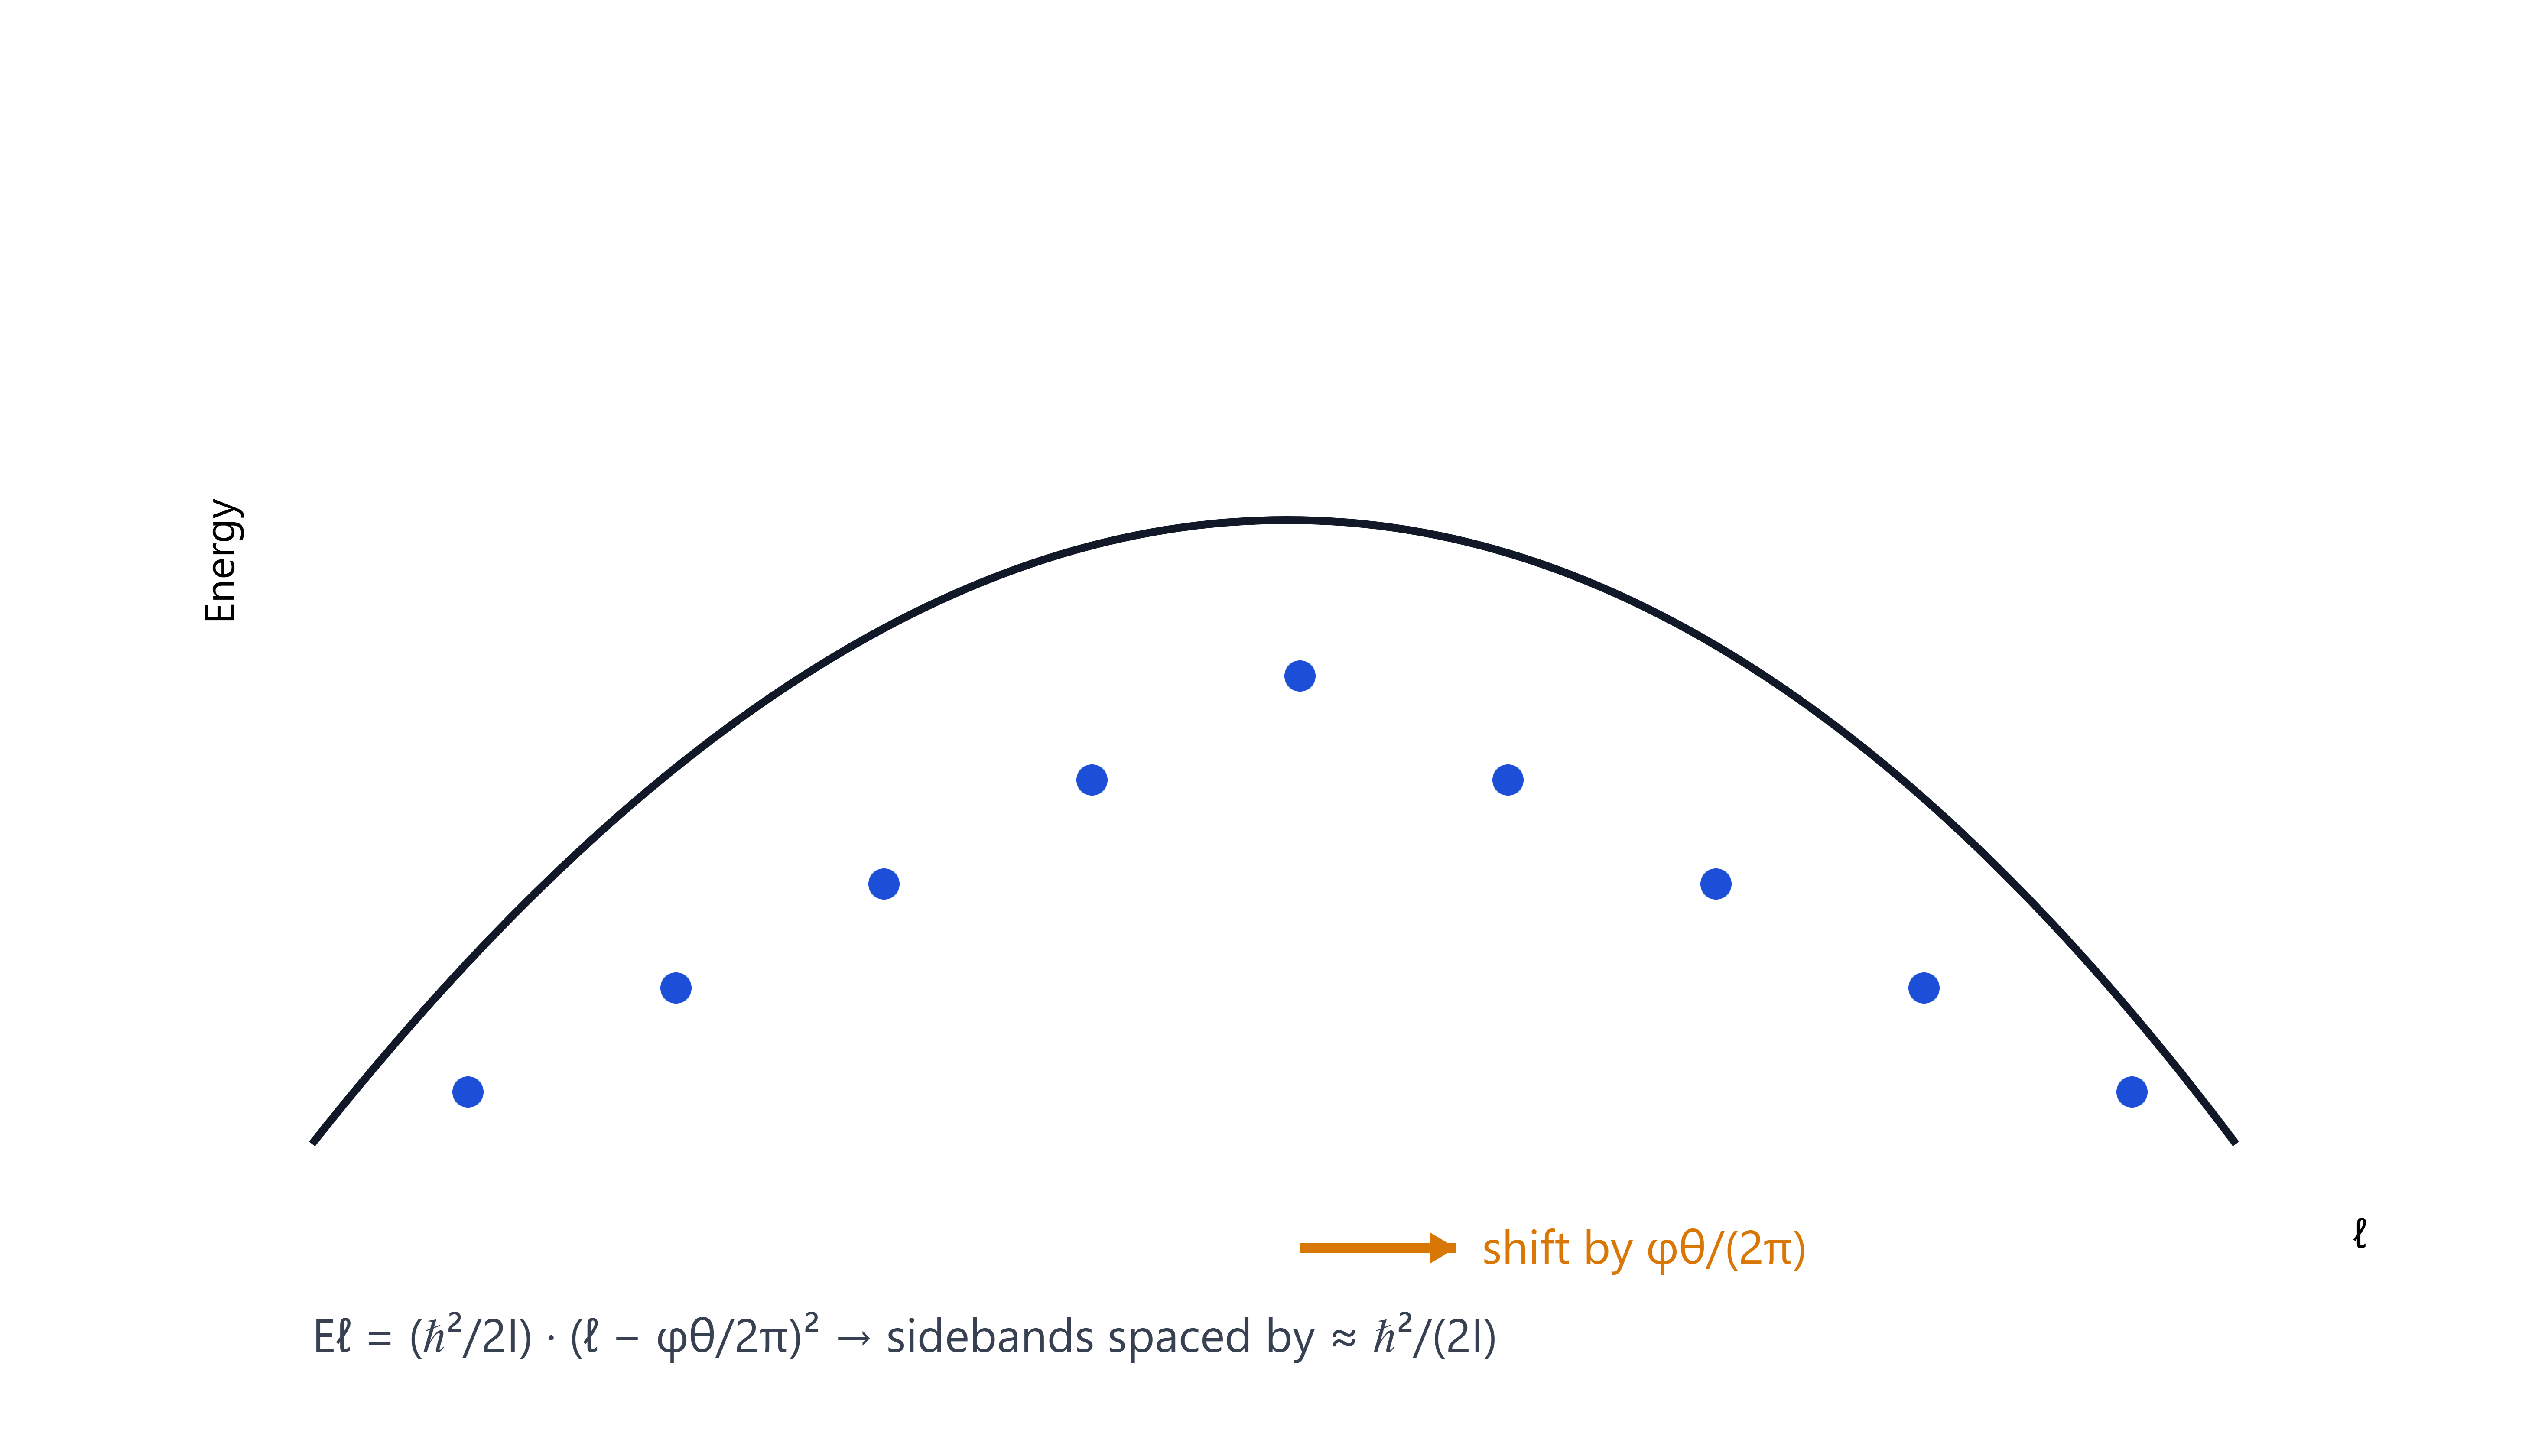
\includegraphics[width=\linewidth]{UG_S3_rotor_ladder.png}
  \caption{Rotor ladder with holonomy shift: the minimum moves by $\phi_\theta/2\pi$.}
  \label{fig:ug-rotor}
\end{figure}

\begin{figure}[htbp]
  \centering
  \begin{subfigure}[b]{0.48\linewidth}
    \centering
    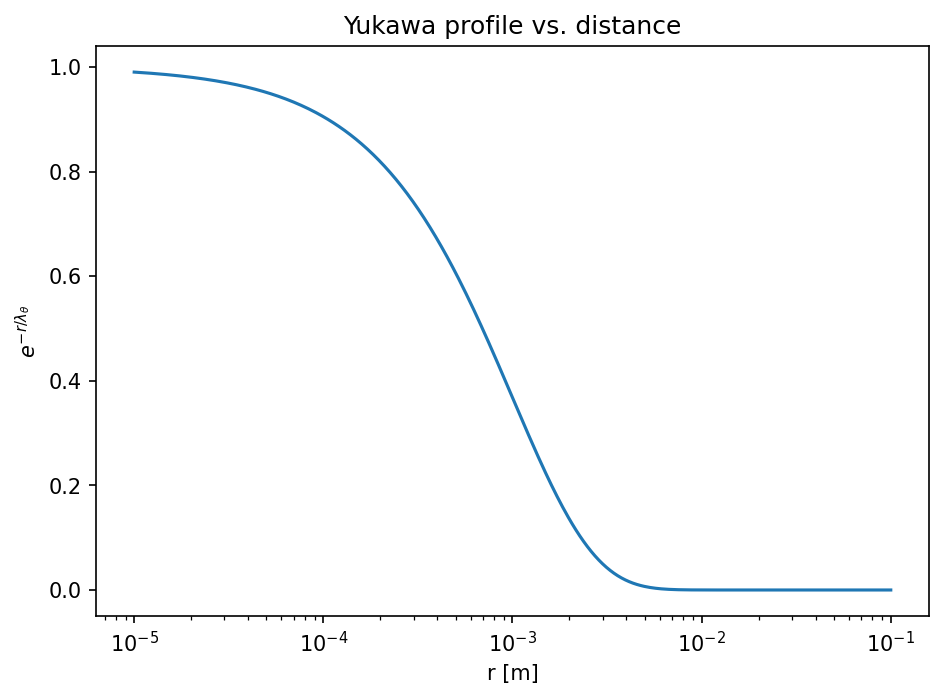
\includegraphics[width=\linewidth]{exp5_yukawa_profile.png}
    \caption{Yukawa profile $V(r)$}
    \label{fig:yukawa-profile}
  \end{subfigure}\hfill
  \begin{subfigure}[b]{0.48\linewidth}
    \centering
    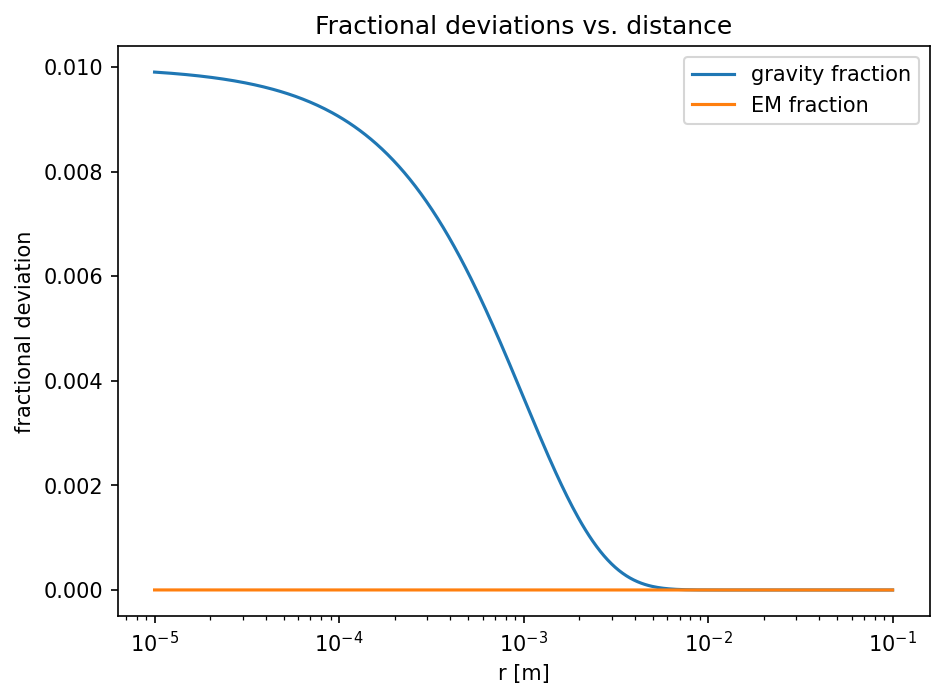
\includegraphics[width=\linewidth]{exp5_fractional_deviation.png}
    \caption{Fractional deviation vs distance}
    \label{fig:yukawa-deviation}
  \end{subfigure}
  \caption{Shared-range $\lambda_\theta$ across sectors.}
  \label{fig:yukawa}
\end{figure}
